%% appendix.tex
%%

%% ==============================
%\chapter{Appendix}
%\label{ch:Appendix}
%% ==============================

\appendix

\iflanguage{english}
{\addchap{Annex}}	% english style
{\addchap{Anhang}}	% german style

\setcounter{figure}{0}


\section{ORCA air coil script}
\label{ch:appendix:sec:orcaScript}
\begin{verbatim}
// import functions for SDS hardware access

#import "~/katrin/ORCARunControl/libs/SDS_RunControl.lib"

#import "~/katrin/ORCARunControl/libs/SDS_AirCoils.lib"



function main(){

//ramp through tenths of the maximum air coil values

for(a=0;a<11; a++){

max=70;

//queue coils 1, 13 and 14 (70A max)

queueAirCoilCurrent_A(1,a*max/10);

queueAirCoilCurrent_A(13,a*max/10);

queueAirCoilCurrent_A(14,a*max/10);

max=100;

//queue coils 2 - 12 (100A max)

for(i=2;i<13;i++){

queueAirCoilCurrent_A(i, a*max/10);

}

//set queued values

sendQueue();

//wait till set

sleep(300);

//output of values

print readAllAirCoilCurrents_A();

sleep(1500);

}

// send the queue of all set points



}
\label{}
\end{verbatim}

\clearpage
\section{Connection scheme DAQ \& high voltage settings}

    \begin{table}[h]
  \centering
  	\begin{tabular}{|c|c|c|c|c|c|}
  	\hline
  		V0 & I0 & I1 & V1 & Ramp Up & Ramp Down\\
  		\hline
  		\SI{1.5}{\kilo\volt} or \SI{1.6}{\kilo\volt} & \SI{2000}{\milli\ampere} & & & \SI{50}{\volt} & \SI{100}{\volt}\\
  		\hline
  	\end{tabular}
  	\caption[High voltage settings]{High voltage settings as used for the muon modules. Modules XX and XX are set to \SI{1.6}{\kilo\volt}.}
  	\label{tab:HVSettings}
  \end{table}
\begin{table}[h]
  	\centering
  	\begin{tabular}{| l | c c | c c | c c | c c |}
  	\hline
  		Module	& 1A	& 1B	& 2A	& 2B	& 3A	& 3B	& 4A	& 4B 	\\
  		Card	& 3	& 3	& 3	& 3	& 6	& 6	& 6	& 6	\\
  		Channel	& 0	& 14	& 3	& 7	& 0	& 14	& 3	& 7	\\
  		HV		& W0 & W1 & W2 & W3 & W4 & W5 & W6 & W7 \\
  		\hline \hline
  		Module	&5A	& 5B	& 6A	& 6B	& 7A	& 7B	& 8A	& 8B	\\
  		Card	& 6	& 6	& 8	& 8	& 8	& 8	& 8	& 8	\\
  		Channel	& 9	& 23	& 0	& 14	& 3	& 7	& 9	& 23	\\
  		HV		& W8 & W9 & E0 & E1 & E2 & E3 & E4 & E5\\
  		\hline
  	\end{tabular}
  	
  	\caption[Main spectrometer DAQ channel assignment]{Assignment of main spectrometer module sides to FLT cards and their channels.}
  	\label{tab:connectionsModulesCards}
  \end{table}
  \begin{figure}[H]
	\centering
  	\includegraphics[width = \textwidth]{graphics/muonModules/mainSpec/FLTback.png}
  	\caption[FLT connector card]{One of the connector cards used at the muon DAQ. The overlayn numbers correspond to the channels accessed via the corresponding connector. Note the non trivial behaviour on le left end. The white labels A, B and C mark the channels used for connecting the muon modules.}
  	\label{fig:FLTback}
  \end{figure}
  

\clearpage
% 
% \begin{figure}
% \centering
% 	\includegraphics[width = 0.9\textwidth]{graphics/monSpec/nonAxiallySym/{+50_12.5_12.5}.eps}
% 	\caption[\SI{50}{\ampere} loops]{Two horizontal loops at \SI{50}{\ampere} current. For all settings see \ref{tab:analysis:nonAxiallySymmetricField}, line 1.}
% 	\label{fig:nonAxiallySym:+50_12.5_12.5.eps}
% \end{figure}
% 
% \begin{figure}
% \centering
% 	\includegraphics[width = 0.9\textwidth]{graphics/monSpec/nonAxiallySym/{+50_12.5_12.5}.eps}
% 	\caption[\SI{50}{\ampere} loops]{Two horizontal loops at \SI{50}{\ampere} current. For all settings see \ref{tab:analysis:nonAxiallySymmetricField}, line 1.}
% 	\label{fig:nonAxiallySym:+50_12.5_12.5.eps}
% \end{figure}
% 
% \begin{figure}
% \centering
% 	\includegraphics[width = 0.9\textwidth]{graphics/monSpec/nonAxiallySym/{+50_12.5_12.5}.eps}
% 	\caption[\SI{50}{\ampere} loops]{Two horizontal loops at \SI{50}{\ampere} current. For all settings see \ref{tab:analysis:nonAxiallySymmetricField}, line 1.}
% 	\label{fig:nonAxiallySym:+50_12.5_12.5.eps}
% \end{figure}


\section{Weather data Christmas 2012}
\label{ch:appendix:sec:weather}

\begin{table}[h]
	\begin{tabular}{| l | cc | cc| cc |}
	\hline
	Date & T$_{low}$ [K] & T$_{high}$ [K] & p$_{low}$ [kPa] & p$_{high}$ [kPa] & p$_l$ / T$_l$ & p$_h$ / T $_h$ \\
	\hline
	21.12.12 & 274.95 & 281.25 & 1010.10 & 1018.20 & 3.67 & 3.62\\
	22.12.12 & 278.55 & 282.15 & 1009.50 & 1020.60 & 3.62 & 3.62\\
	23.12.12 & 282.85 & 287.25 & 1009.50 & 1013.70 & 3.57 & 3.53\\
	24.12.12 & 277.05 & 287.15 & 1007.40 & 1013.50 & 3.64 & 3.53\\
	25.12.12 & 276.05 & 288.35 & 1004.00 & 1010.30 & 3.64 & 3.50\\
	26.12.12 & 281.25 & 282.85 & 1010.40 & 1016.40 & 3.59 & 3.59\\
	27.12.12 & 280.75 & 283.25 & 1004.80 & 1014.70 & 3.58 & 3.58\\
	28.12.12 & 279.65 & 281.85 & 1016.20 & 1029.50 & 3.63 & 3.65\\
	29.12.12 & 276.05 & 284.55 & 1014.90 & 1026.00 & 3.68 & 3.61\\
	30.12.12 & 279.05 & 282.85 & 1015.90 & 1024.60 & 3.64 & 3.62\\
	31.12.12 & 277.05 & 283.15 & 1011.60 & 1024.40 & 3.65 & 3.62\\
	01.01.13 & 274.45 & 281.45 & 1008.10 & 1016.90 & 3.67 & 3.61\\
	02.01.13 & 272.25 & 279.15 & 1017.50 & 1033.00 & 3.74 & 3.70\\
	03.01.13 & 273.65 & 280.45 & 1033.10 & 1038.30 & 3.78 & 3.70\\
	\hline
	
	\end{tabular}
	\caption[Temperature and pressure Rheinstetten]{Temperature and pressure data from the weather station in Rheinstetten. Daily high and low were given, included are the ratio of pressure and temperature for both the high and the low values. This ratio is proportional to the air's density . Bare in mind that this data is only for the low atmospheric layer and the station is also around \SI{20}{\kilo\meter} away  from the KATRIN muon modules.}
	\label{fig:weatherData}
\end{table}

\clearpage


\section{Other monitor spectrometer settings}
\label{ch:appendix:sec:monSpec}

\begin{table}[h]
			\begin{tabular}{C{\textwidth}}
			{\bf non-axially symmetric magnetic field}\\
		\end{tabular}\\
		\begin{tabularx}{\textwidth}{|>{\centering}X>{\centering}X>{\centering}X>{\centering}X>{\centering}X>{\centering}X>{\centering\arraybackslash}X|}
			\hline
			\centering
			solenoid source &solenoid detector &inner aircoil & outer aircoil &outer cent. aircoil &emcs x	&emcs y\\
			\hline
			25	&25	&7	&-7	&5	&0	&-14\\
			\hline
		\end{tabularx}
		\begin{tabularx}{\textwidth}{|l|X|}
		\hline
			mos00159753- & Two horizontal loops at \SI{100}{\ampere}\\
			mos00159754 &\\
			\hline
			mos00159755-& Two horizontal loops at \SI{-100}{\ampere}\\
			mos00159758 &\\
			\hline
			mos00159759-& No current in horizontal loops - background measurement\\
			mos00159771 &\\
			\hline
			mos00159772-& Two horizontal loops at \SI{100}{\ampere}\\
			mos00159773 &\\
			\hline
		\end{tabularx}
		\vspace{0.5cm}
		
		\begin{tabularx}{\textwidth}{|>{\centering}X>{\centering}X>{\centering}X>{\centering}X>{\centering}X>{\centering}X>{\centering\arraybackslash}X|}
			\hline
			\centering
			solenoid source &solenoid detector &inner aircoil & outer aircoil &outer cent. aircoil &emcs x	&emcs y\\
			\hline
			12.5	&12.5	&3.5	&-3.5	&2.5	&0	&0\\
			\hline
		\end{tabularx}
		\begin{tabularx}{\textwidth}{|l|X|}
			\hline
			mos00160661- & Two horizontal loops at \SI{50}{\ampere}\\
			mos00160666 &\\
			\hline
			mos00160667-&No current in horizontal loops - background measurement\\
			mos00160682 &\\
			\hline
			mos00160684-& Two horizontal loops at \SI{-50}{\ampere}\\
			mos00160687 &\\
			\hline
		\end{tabularx}
		\vspace{0.5cm}
		
		\begin{tabularx}{\textwidth}{|>{\centering}X>{\centering}X>{\centering}X>{\centering}X>{\centering}X>{\centering}X>{\centering\arraybackslash}X|}
			\hline
			\centering
			solenoid source &solenoid detector &inner aircoil & outer aircoil &outer cent. aircoil &emcs x	&emcs y\\
			\hline
			6.2 & 6.2 & 1.7 & -1.7 & 1.2 & 0 & 0\\
			\hline
		\end{tabularx}
				\begin{tabularx}{\textwidth}{|l|X|}
			\hline
			mos00160688- & Two horizontal loops at \SI{25}{\ampere}\\
			mos00160691 &\\
			\hline
			mos00160692-&No current in horizontal loops - background measurement\\
			mos00160706 &\\
			\hline
			mos00160707-& Two horizontal loops at \SI{-25}{\ampere}\\
			mos00160711 &\\
			\hline
		\end{tabularx}
\end{table}

% \begin{figure}
% \centering
% 	\includegraphics[width = 0.9\textwidth]{graphics/monSpec/nonAxiallySym/{+50_12.5_12.5}.eps}
% 	\caption[\SI{50}{\ampere} loops]{Two horizontal loops at \SI{50}{\ampere} current. For all settings see \ref{tab:analysis:nonAxiallySymmetricField}, line 1.}
% 	\label{fig:nonAxiallySym:+50_12.5_12.5.eps}
% \end{figure}
% 
% \begin{figure}
% \centering
% 	\includegraphics[width = 0.9\textwidth]{graphics/monSpec/nonAxiallySym/{-50_12.5_12.5}.eps}
% 	\caption[\SI{-50}{\ampere} loops]{Two horizontal loops at \SI{-50}{\ampere} current. For all settings see \ref{tab:analysis:nonAxiallySymmetricField}, line 3.}
% 	\label{fig:nonAxiallySym:-50_12.5_12.5.eps}
% \end{figure}
% 
% \begin{figure}
% \centering
% 	\includegraphics[width = 0.9\textwidth]{graphics/monSpec/nonAxiallySym/{+25_12.5_12.5}.eps}
% 	\caption[\SI{25}{\ampere} loops]{Two horizontal loops at \SI{25}{\ampere} current. For all settings see \ref{tab:analysis:nonAxiallySymmetricField}, line 2.}
% 	\label{fig:nonAxiallySym:+25_12.5_12.5.eps}
% \end{figure}
% \begin{figure}
% \centering
% 	\includegraphics[width = 0.9\textwidth]{graphics/monSpec/nonAxiallySym/{-25_12.5_12.5}.eps}
% 	\caption[\SI{-25}{\ampere} loops]{Two horizontal loops at \SI{-25}{\ampere} current. For all settings see \ref{tab:analysis:nonAxiallySymmetricField}, line 4.}
% 	\label{fig:nonAxiallySym:-25_12.5_12.5.eps}
% \end{figure}
% \begin{figure}
% \centering
% 	\includegraphics[width = 0.9\textwidth]{graphics/monSpec/nonAxiallySym/{BG_12.5_12.5}.eps}
% 	\caption[\SI{50}{\ampere} loops]{Two horizontal loops at \SI{0}{\ampere} current. For all settings see \ref{tab:analysis:nonAxiallySymmetricField}, line 1.}
% 	\label{fig:nonAxiallySym:BG_12.5_12.5.eps}
% \end{figure}
% 
% \begin{figure}
% \centering
% 	\includegraphics[width = 0.9\textwidth]{graphics/monSpec/nonAxiallySym/{BG_25_25}.eps}
% 	\caption[\SI{50}{\ampere} loops]{}
% 	\label{fig:nonAxiallySym:BG_25_25.eps}
% \end{figure}
% 
\clearpage

%%%%%%%%%%%%%%%%%%%%%%%%%%%%%%%%%%%
%MonSpec
%%%%%%%%%%%%%%%%%%%%%%%%%%%%%%%%%%%%
\section{Monitor spectrometer field setup and analysis}
\label{ch:appendix:sec:A3}


\begin{figure}[H]
\centering

		\centerline{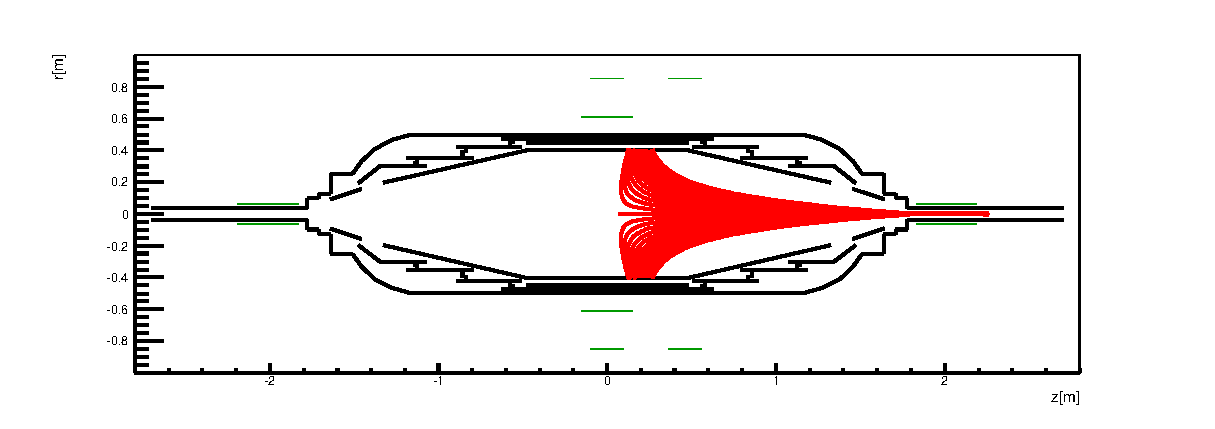
\includegraphics[width = 1.3\linewidth]{graphics/analysis/monSpec/fieldSimulation/AB.eps} }
	
	\caption[Asymmetric field \SI{50}{\ampere}]{Flux tube for a \SI{50}{\ampere} detector solenoid, \SI{-8}{\ampere} outer central air coil current.}
	\label{fig:ABf}

\centering
	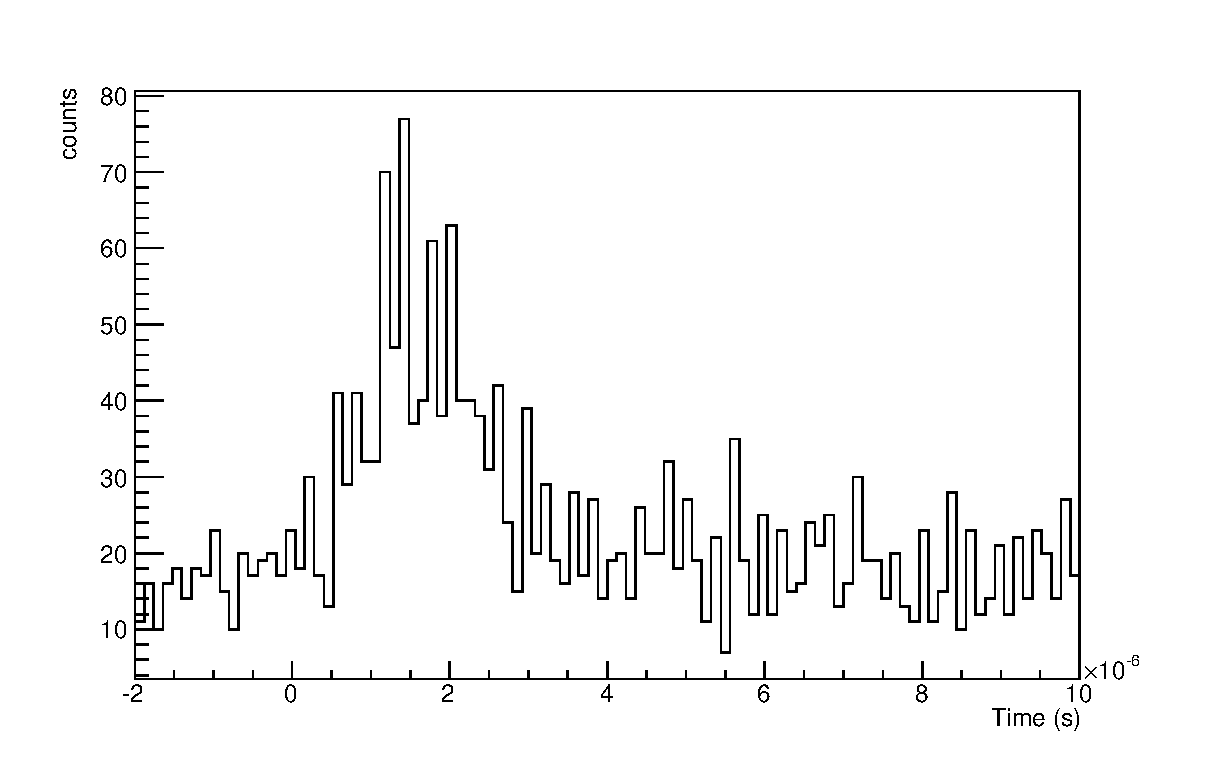
\includegraphics[width = 0.9\textwidth]{graphics/analysis/monSpec/AB.eps}
	\caption[\SI{50}{\ampere} loops]{Source solenoid off, detector solenoid at \SI{25}{\ampere}. A peak in time is visible at \SI{1.8}{\micro\second}. }
	\label{fig:AB}
\end{figure}

\clearpage

\begin{figure}[H]
\centering
			\centerline{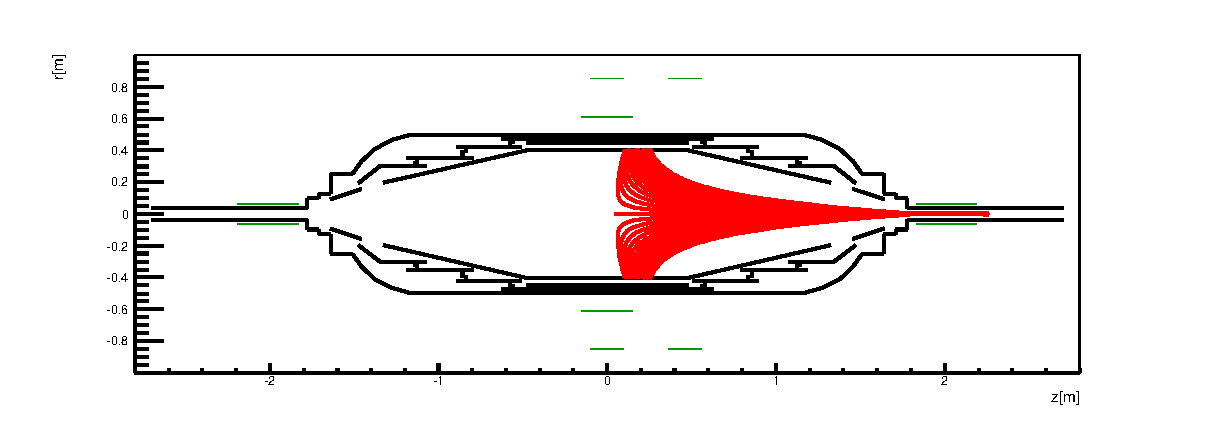
\includegraphics[width = 1.3\linewidth]{graphics/analysis/monSpec/fieldSimulation/AA.eps}}
	
	\caption[\SI{25}{\ampere} asymmetric]{Flux tube for a \SI{25}{\ampere} detector solenoid.}
	\label{fig:AAf}
\end{figure}

\begin{figure}
\centering
	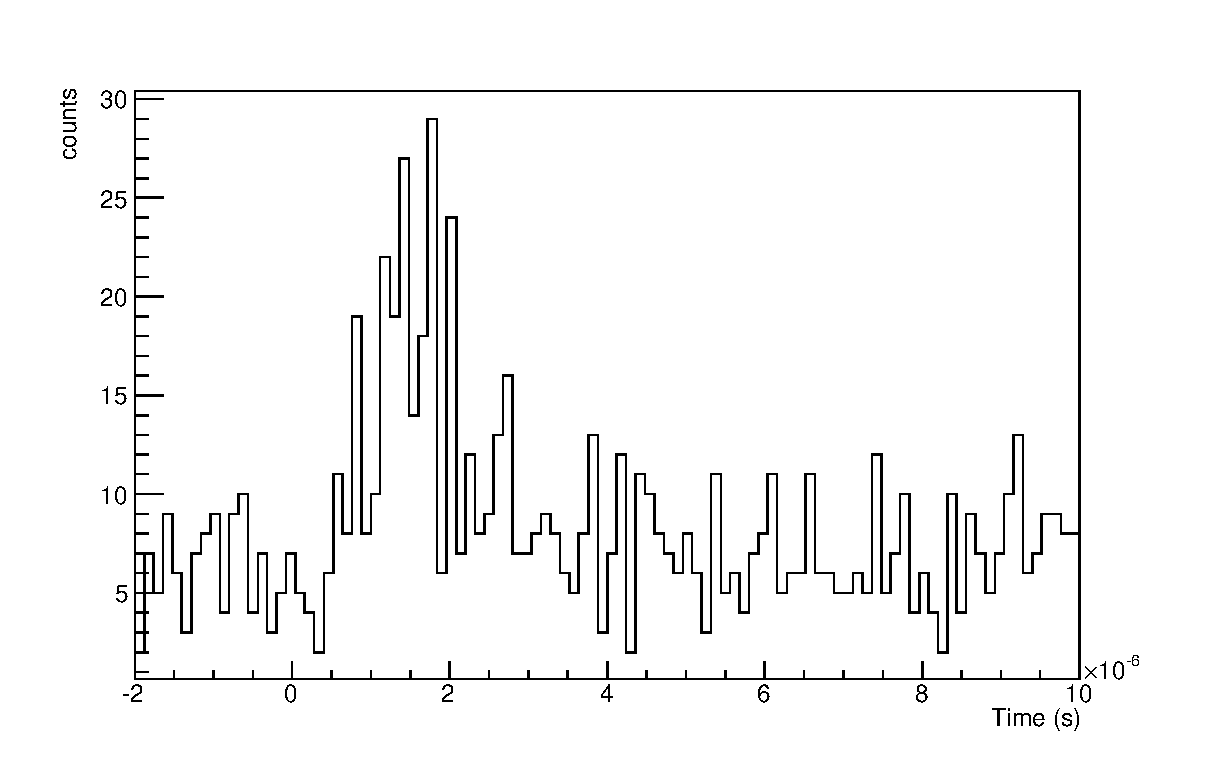
\includegraphics[width = 0.9\textwidth]{graphics/analysis/monSpec/AA.eps}
	\caption[\SI{25}{\ampere} asymmetric]{Source solenoid off, detector solenoid at \SI{25}{\ampere}}.
	\label{fig:AA}
\end{figure}
\clearpage



\begin{figure}
\centering
	\centerline{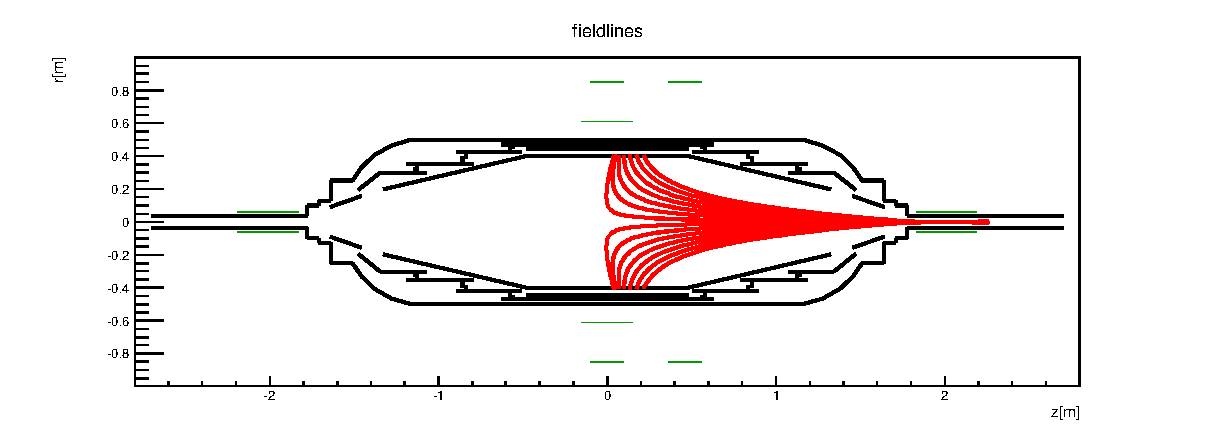
\includegraphics[width = 1.3\linewidth]{graphics/analysis/monSpec/fieldSimulation/AC.eps} }
	
	\caption[\SI{50}{\ampere} loops]{Flux tube for a \SI{50}{\ampere} detector solenoid, \SI{-7}{\ampere} outer central air coil current.}
	\label{fig:ACf}
\end{figure}

\begin{figure}
\centering
	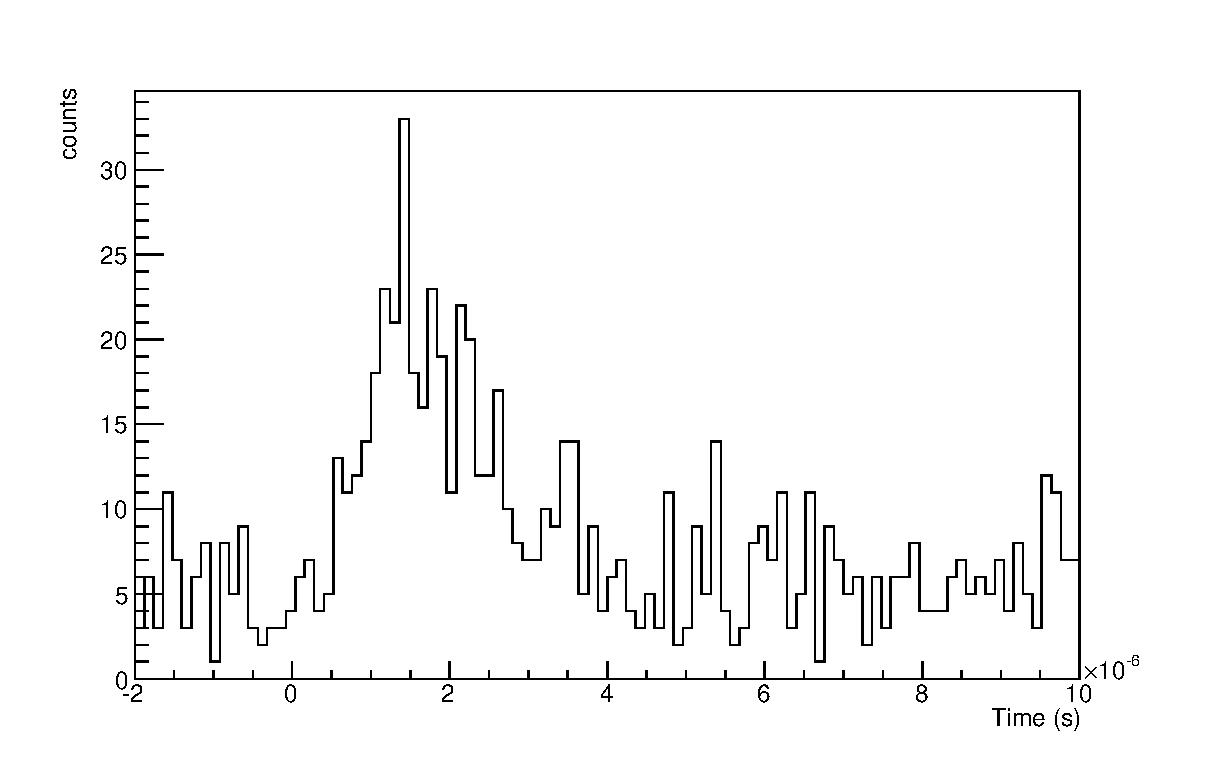
\includegraphics[width = 0.9\textwidth]{graphics/analysis/monSpec/AC.eps}
	\caption[\SI{50}{\ampere} loops]{Two horizontal loops at \SI{0}{\ampere} current. Both solenoids at \SI{25}{\ampere}.}
	\label{fig:AC}
\end{figure}
\clearpage






\begin{figure}
\centering
	\centerline{\includegraphics[width = 1.3\linewidth]{graphics/analysis/monSpec/fieldSimulation/AD.eps} }
	
	\caption[\SI{50}{\ampere} loops]{Flux tube for a \SI{50}{\ampere} detector solenoid, \SI{-6}{\ampere} outer central air coil current.}
	\label{fig:ADf}
\end{figure}

\begin{figure}
\centering
	\includegraphics[width = 0.9\textwidth]{graphics/analysis/monSpec/AD.eps}
	\caption[\SI{50}{\ampere} loops]{Two horizontal loops at \SI{0}{\ampere} current. Both solenoids at \SI{25}{\ampere}.}
	\label{fig:AD}
\end{figure}
\clearpage









\begin{figure}
\centering
	\centerline{\includegraphics[width = 1.3\linewidth]{graphics/analysis/monSpec/fieldSimulation/NA.eps} }
	
	\caption[\SI{0}{\ampere} loops]{Two horizontal loops at \SI{0}{\ampere} current. Both solenoids at \SI{25}{\ampere} for a comparison of the background at different field widening.}
	\label{fig:NAf}
\end{figure}

\begin{figure}
\centering
	\includegraphics[width = 0.9\textwidth]{graphics/analysis/monSpec/NA.eps}
	\caption[\SI{0}{\ampere} loops analysis]{Two horizontal loops at \SI{0}{\ampere} current. Both solenoids at \SI{25}{\ampere} for a comparison of the background at different field widening. Some events occur in the expected time window.}
	\label{fig:NA}
\end{figure}
\clearpage



\begin{figure}
\centering
	\centerline{\includegraphics[width = 1.3\linewidth]{graphics/analysis/monSpec/fieldSimulation/NI.eps} }
	
	\caption[\SI{0}{\ampere} loops]{Two horizontal loops at \SI{0}{\ampere} current. Both solenoids at \SI{12.5}{\ampere} for a comparison of the background at different field widening. }
	\label{fig:NIf}
\end{figure}

\begin{figure}
\centering
	\includegraphics[width = 0.9\textwidth]{graphics/analysis/monSpec/NI.eps}
	\caption[\SI{0}{\ampere} loops analysis]{Two horizontal loops at \SI{0}{\ampere} current. Both solenoids at \SI{12.5}{\ampere} for a comparison of the background at different field widening.}
	\label{fig:NI}
\end{figure}
\clearpage



\begin{figure}
\centering
	\centerline{\includegraphics[width = 1.3\linewidth]{graphics/analysis/monSpec/fieldSimulation/NB.eps} }
	
	\caption[\SI{50}{\ampere} loops]{Two horizontal loops at \SI{50}{\ampere} current. Both solenoids at \SI{12.5}{\ampere}. Shift of the flux tube downwards visible.}
	\label{fig:NBf}
\end{figure}

\begin{figure}
\centering
	\includegraphics[width = 0.9\textwidth]{graphics/analysis/monSpec/NB.eps}
	\caption[\SI{50}{\ampere} loops analysis]{Two horizontal loops at \SI{50}{\ampere} current. Both solenoids at \SI{12.5}{\ampere} }
	\label{fig:NB}
\end{figure}
\clearpage





\begin{figure}
\centering
	\centerline{\includegraphics[width = 1.3\linewidth]{graphics/analysis/monSpec/fieldSimulation/NE.eps} }
	
	\caption[\SI{-50}{\ampere} loops]{Two horizontal loops at \SI{-50}{\ampere} current. Both solenoids at \SI{12.5}{\ampere}. Shift of the flux tube upwards visible.}
	\label{fig:NEf}
\end{figure}

\begin{figure}
\centering
	\includegraphics[width = 0.9\textwidth]{graphics/analysis/monSpec/NE.eps}
	\caption[\SI{-50}{\ampere} loops analysis]{Two horizontal loops at \SI{-50}{\ampere} current. Both solenoids at \SI{12.5}{\ampere}.}
	\label{fig:NE}
\end{figure}
\clearpage





\begin{figure}
\centering
	\centerline{\includegraphics[width = 1.3\linewidth]{graphics/analysis/monSpec/fieldSimulation/NC.eps} }
	
	\caption[\SI{25}{\ampere} loops]{Two horizontal loops at \SI{25}{\ampere} current. Both solenoids at \SI{12.5}{\ampere}. Shift of the flux tube downwards visible.}
	\label{fig:NCf}
\end{figure}

\begin{figure}
\centering
	\includegraphics[width = 0.9\textwidth]{graphics/analysis/monSpec/NC.eps}
	\caption[\SI{25}{\ampere} loops]{Two horizontal loops at \SI{25}{\ampere} current. Both solenoids at \SI{12.5}{\ampere}.}
	\label{fig:NC}
\end{figure}
\clearpage








\begin{figure}
\centering
	\centerline{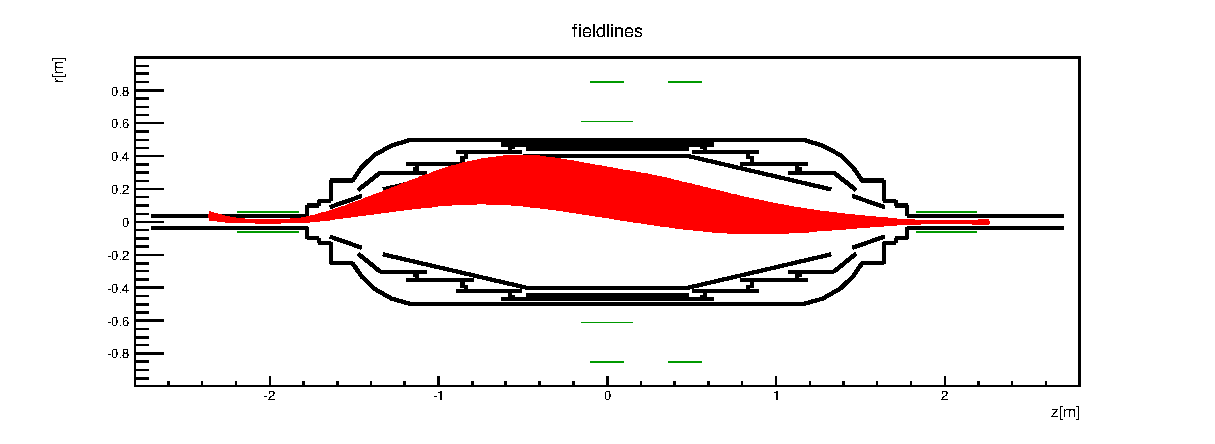
\includegraphics[width = 1.3\linewidth]{graphics/analysis/monSpec/fieldSimulation/ND.eps} }
	
	\caption[\SI{50}{\ampere} loops]{Two horizontal loops at \SI{-25}{\ampere} current. Both solenoids at \SI{25}{\ampere}. Shift of the flux tube upwards visible. }
	\label{fig:NDf}
\end{figure}

\begin{figure}
\centering
	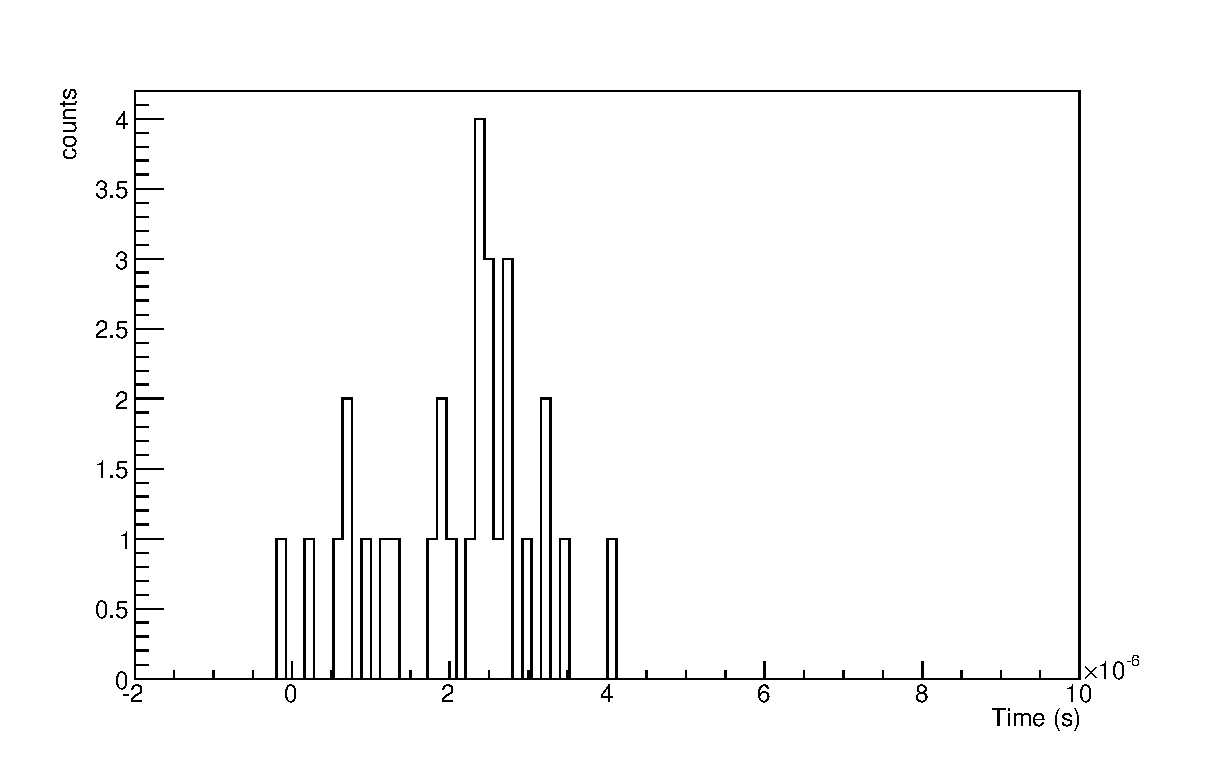
\includegraphics[width = 0.9\textwidth]{graphics/analysis/monSpec/ND.eps}
	\caption[\SI{50}{\ampere} loops]{Two horizontal loops at \SI{-25}{\ampere} current. Both solenoids at \SI{25}{\ampere}. Unexpectedly low counts probably due to a off-detector flux tube. }
	\label{fig:ND}
\end{figure}
\clearpage











\section{Main spectrometer analysis}
\label{ch:appendix:sec:mainSpec}


\section{A vis.mac file}
\label{ch:appendix:sec:vis.mac}

\begin{verbatim}
# Macro file for the visualization setting in the initialization phase 
# of the Geant4 simulation when running in interactive mode
#
# Use this open statement to create an OpenGL view:
/vis/open OGL 600x600-0+0
#
# Disable auto refresh and quieten vis messages whilst scene and
# trajectories are established:
/vis/viewer/set/autoRefresh false
/vis/verbose warnings
#
# Draw geometry:
/vis/drawVolume
#
# Specify view angle and zoom:
/vis/viewer/set/viewpointVector 0 0 1
#/vis/viewer/set/viewpointThetaPhi 40 40
/vis/viewer/zoomTo 2
#
# Specify style (surface, wireframe, auxiliary edges, display limit...)
/vis/viewer/set/style wireframe
/vis/viewer/set/auxiliaryEdge true
/vis/ogl/set/displayListLimit 100000000
#
# Draw smooth trajectories at end of event, showing trajectory points
# as markers 1 pixel wide:
/vis/scene/add/trajectories smooth
/vis/modeling/trajectories/create/drawByCharge
/vis/modeling/trajectories/drawByCharge-0/default/setDrawStepPts true
/vis/modeling/trajectories/drawByCharge-0/default/setStepPtsSize 1
#
# Draw hits at end of event:
/vis/scene/add/hits
#
# To draw only muons:
/vis/filtering/trajectories/create/particleFilter
/vis/filtering/trajectories/particleFilter-0/add mu+
# To superimpose all of the events from a given run:
/vis/scene/endOfEventAction accumulate
#
# Re-establish auto refreshing and verbosity:
/vis/viewer/set/autoRefresh true
/vis/viewer/set/background grey
/vis/viewer/set/projection perspective
/vis/verbose warnings
#
#Generate 5 muon events with the distribution provided in the code
/run/beamOn 5

\end{verbatim}


